\chapter{Previsão do prêmio de risco de volatilidade}
\label{chap:previsao_bvrp}

Este capítulo prevê o BVRP fora da amostra, apenas com a informação disponível
em $t$. A previsão é necessária porque a versão do prêmio conhecida em $t$, a
$\text{BVRP}^{\text{proxy}}$, tem correlação de $-0{,}02$ com o BVRP na mesma
data (Seção~\ref{sec:met-variaveis}): a hipótese de passeio aleatório sem
deriva para a volatilidade histórica aproxima mal a realização do prêmio. O
BVRP previsto aqui é o regressor dos Capítulos~\ref{chap:retornos_linear}
e~\ref{chap:retornos_nao_linear}.

Na janela expansiva, os cinco modelos superam a média histórica fora da
amostra. O melhor, o Ridge,
reduz o erro quadrático em 22\%, e o teste de \citet{clark2007approximately}
rejeita a igualdade com a média para quatro dos cinco modelos, mesmo com a
correção de Bonferroni. A previsibilidade, porém, é modesta: o teste de
\citet{diebold1995comparing} não rejeita depois da correção, as previsões ficam
próximas da média e nenhum modelo antecipa os episódios de prêmio positivo. As
duas referências ingênuas, a proxy e o prêmio realizado defasado, erram mais
que a média. A relação entre as variáveis e o prêmio muda com o regime de
volatilidade dentro da amostra, primeira evidência de não linearidade, mas
essa mudança não melhora a previsão fora dela.

% =========================================================
\section{Alvo e informação disponível}
\label{sec:prev-alvo}

O alvo é o prêmio da janela de 30 dias que começa no dia seguinte à previsão:
\begin{equation}
\text{BVRP}_{t+1:t+30\,|\,t} = \text{VH}_{t+1:t+30} - \text{IV}_t = f(X_t) + u_t,
\label{eq:prev-alvo}
\end{equation}
em que $X_t$ reúne as variáveis explicativas conhecidas no fim do dia $t$
(Seção~\ref{sec:prev-variaveis}). O índice $t+1:t+30\,|\,t$ separa a janela da
volatilidade histórica e a data da informação. Trata-se do mesmo
$\text{BVRP}_t$ dos capítulos anteriores, sem deslocamento para $t+1$: a
previsão feita em $t$ é comparada com o prêmio cuja IV é a de $t$, e não com o
prêmio de $t+1$. A equação~\eqref{eq:prev-alvo} é a
equação~\eqref{eq:met-previsao-bvrp} com a janela explícita; o restante do
texto usa $\text{BVRP}_t$.

Como o alvo de $s$ só se realiza em $s+30$, o modelo da origem $t$ usa apenas
as datas $s \le t - 30$. As previsões cobrem 987 datas, de 21/06/2023 a
03/03/2026, em 33 origens com reestimação a cada 30 dias; o treino tem de 760
observações, na primeira origem, a 1.720, na última (janela expansiva). A
janela móvel, de 730 observações, serve de teste de robustez
(Seção~\ref{sec:met-amostras}).

% =========================================================
\section{Variáveis explicativas}
\label{sec:prev-variaveis}

A Tabela~\ref{tab:prev-dicionario} lista as 17 variáveis explicativas, em
quatro grupos. As volatilidades históricas de 1, 5 e 30 dias seguem a estrutura
do modelo HAR de \citet{corsi2009har}, com componentes diário, semanal e
mensal; as de 60 e 90 dias estendem essa estrutura para horizontes mais
longos. A IV entra em nível, em variação de 1 e 5 dias e como desvio em relação
às médias móveis de 5 e 30 dias. O preço entra por log-retornos de 1, 5 e 30
dias e pela razão com a média móvel de 30 dias. O último grupo traz a proxy, sua
variação diária e o prêmio realizado defasado, $\text{BVRP}_{t-30} =
\text{VH}_{t-29:t} - \text{IV}_{t-30}$, o prêmio mais recente já realizado em
$t$. Ele é igual à proxy mais a variação da IV em 30 dias,
$\text{IV}_t - \text{IV}_{t-30}$.

O tratamento segue os testes de raiz unitária. O preço e as médias móveis da IV,
em que o ADF não rejeita a raiz unitária e o KPSS rejeita a estacionariedade,
entram transformados. As volatilidades
entram em nível, mesmo quando o teste ADF fica na fronteira, como na
volatilidade histórica de 90 dias ($p = 0{,}19$) e na IV ($p = 0{,}08$): em
janelas móveis longas, observações vizinhas compartilham quase todos os
retornos (89 de 90 dias), o que gera persistência mecânica e reduz o poder do
teste. Como $\text{BVRP}^{\text{proxy}}_t = \text{VH}_{t-29:t} - \text{IV}_t$,
os modelos lineares excluem a volatilidade histórica de 30 dias; as árvores
usam as 17 variáveis.

As variáveis já trazem não linearidade em relação aos retornos diários. A
volatilidade histórica é a raiz da média dos retornos ao quadrado; a de 1 dia
é o valor absoluto do retorno. Os modelos lineares, portanto, são lineares nas
variáveis construídas, e não nos retornos.

\begin{table}[H]
\centering
\scriptsize
\caption{Variáveis explicativas, todas conhecidas no fim do dia $t$.}
\label{tab:prev-dicionario}
\begin{tabular}{lp{4.2cm}lrl}
\toprule
Símbolo & Definição & Código & ADF ($p$) & Tratamento \\
\midrule
\multicolumn{5}{l}{\textit{Volatilidade histórica}} \\
$\text{VH}_{t:t}$ & $\sqrt{365}\,|r_t|$ & \texttt{vh\_1d} & $<$0{,}001 & nível \\
$\text{VH}_{t-4:t}$ & $\sqrt{(365/5)\sum_{j=0}^{4} r_{t-j}^2}$ & \texttt{vh\_5d} & $<$0{,}001 & nível \\
$\text{VH}_{t-29:t}$ & $\sqrt{(365/30)\sum_{j=0}^{29} r_{t-j}^2}$ & \texttt{vh\_30d} & $<$0{,}001 & nível \\
$\text{VH}_{t-59:t}$ & idem, 60 dias & \texttt{vh\_60d} & 0{,}028 & nível \\
$\text{VH}_{t-89:t}$ & idem, 90 dias & \texttt{vh\_90d} & 0{,}190 & nível \\
\addlinespace
\multicolumn{5}{l}{\textit{Volatilidade implícita}} \\
$\text{IV}_t$ & DVOL no fim de $t$ & \texttt{iv\_30d} & 0{,}084 & nível \\
$\Delta_1\text{IV}_t$ & $\text{IV}_t - \text{IV}_{t-1}$ & \texttt{d\_iv\_1d} & $<$0{,}001 & diferença \\
$\Delta_5\text{IV}_t$ & $\text{IV}_t - \text{IV}_{t-5}$ & \texttt{d\_iv\_5d} & $<$0{,}001 & diferença \\
$\text{IV}_t - \overline{\text{IV}}_{t-4:t}$ & desvio da média móvel de 5 dias & \texttt{iv\_menos\_ma5d} & $<$0{,}001 & desvio da média móvel \\
$\text{IV}_t - \overline{\text{IV}}_{t-29:t}$ & desvio da média móvel de 30 dias & \texttt{iv\_menos\_ma30d} & $<$0{,}001 & desvio da média móvel \\
\addlinespace
\multicolumn{5}{l}{\textit{Preço}} \\
$r_t$ & $\ln(P_t/P_{t-1})$ & \texttt{ret\_1d} & $<$0{,}001 & log-diferença do preço \\
$r_{t-4:t}$ & $\sum_{j=0}^{4} r_{t-j}$ & \texttt{ret\_acum\_5d} & $<$0{,}001 & soma de log-diferenças \\
$r_{t-29:t}$ & $\sum_{j=0}^{29} r_{t-j}$ & \texttt{ret\_acum\_30d} & $<$0{,}001 & soma de log-diferenças \\
$\ln(P_t/\overline{P}_{t-29:t})$ & preço relativo à média móvel de 30 dias & \texttt{log\_close\_ma30d} & $<$0{,}001 & razão com a média móvel \\
\addlinespace
\multicolumn{5}{l}{\textit{Prêmio}} \\
$\text{BVRP}^{\text{proxy}}_t$ & $\text{VH}_{t-29:t} - \text{IV}_t$ & \texttt{vrp\_30d} & $<$0{,}001 & nível \\
$\Delta_1\text{BVRP}^{\text{proxy}}_t$ & $\text{BVRP}^{\text{proxy}}_t - \text{BVRP}^{\text{proxy}}_{t-1}$ & \texttt{d\_vrp\_1d} & $<$0{,}001 & diferença \\
$\text{BVRP}_{t-30}$ & $\text{VH}_{t-29:t} - \text{IV}_{t-30}$ & \texttt{bvrp\_realizado\_defasado} & $<$0{,}001 & nível \\
\bottomrule
\end{tabular}
\par\smallskip
\parbox{0.95\linewidth}{\footnotesize\textit{Nota}: $r_t$ é o log-retorno diário e $P_t$, o preço de fechamento. Volatilidades em \% a.a. Valor-$p$ do teste ADF na amostra de modelagem ($N = 1.776$). As séries em que o ADF não rejeita a raiz unitária e o KPSS rejeita a estacionariedade (o preço e as médias móveis da IV) entram transformadas; as volatilidades entram em nível, inclusive $\text{VH}_{t-89:t}$ e $\text{IV}_t$, cujo ADF fica na fronteira. Os modelos lineares excluem $\text{VH}_{t-29:t}$, porque $\text{BVRP}^{\text{proxy}}_t = \text{VH}_{t-29:t} - \text{IV}_t$.}
\end{table}


% =========================================================
\section{Modelos e hiperparâmetros}
\label{sec:prev-modelos}

A dissertação compara cinco modelos para $f$ na
equação~\eqref{eq:prev-alvo}: o MQO; o Ridge \citep{hoerl1970ridge} e o LASSO
\citep{tibshirani1996lasso}, que penalizam os coeficientes do MQO; a floresta
aleatória \citep{breiman2001randomforest}, com 500 árvores; e o XGBoost
\citep{chen2016xgboost}. Os três modelos lineares usam as variáveis
padronizadas com a média e o desvio-padrão do treino de cada origem.

Em cada uma das 33 reestimações, a validação cruzada embargada
\citep{lopezdeprado2018advances} escolhe os hiperparâmetros: cinco dobras
expansivas dentro do treino da origem, em que o treino da dobra termina 30 dias
antes do início da validação, para que nenhum alvo de treino se sobreponha aos
de validação. A validação fica com a combinação de menor erro quadrático médio
nas dobras. A Tabela~\ref{tab:prev-hiperparametros} mostra as grades e as escolhas.

No Ridge e no LASSO, a penalidade escolhida fica sempre no interior da grade. O
LASSO zera todos os coeficientes em 12 das 33 origens; nelas, prevê
exatamente a média histórica do treino. As árvores ficam no extremo de menor
capacidade: a floresta usa árvores de profundidade 1 em todas as origens, e o
XGBoost usa a menor taxa de aprendizagem em todas, profundidade 1 em 28 e o
menor número de árvores em 22. Esse limite não é uma deficiência da grade.
Árvores de um único corte, com aprendizagem lenta, já produzem previsões
próximas da média histórica: o desvio-padrão das previsões fora da amostra é de
2,3 p.p. na floresta e de 2,0 p.p. no XGBoost, contra 4,5 p.p. no Ridge.
Ampliar a grade nessa direção só aproximaria mais as previsões da média. A
validação cruzada prefere, assim, as configurações menos flexíveis da grade,
sinal de que a estrutura não linear que as árvores conseguem extrair é fraca.

\begin{table}[H]
\centering
\small
\caption{Hiperparâmetros: grades e escolhas da validação cruzada embargada.}
\label{tab:prev-hiperparametros}
\begin{tabular}{lp{6.2cm}lc}
\toprule
Modelo & Grade & Mais frequente & No limite \\
\midrule
Ridge & $\alpha$: 17 valores de $10^{-3}$ a $10^{5}$ & $\alpha = 10^{3}$ (24) & 0 \\
LASSO & $\alpha$: 16 valores de $10^{-3}$ a $10^{2}$ & $\alpha = 4{,}64$ (18) & 0 \\
\addlinespace
Floresta aleatória & profundidade máxima: 1, 2, 3, 6, sem limite & 1 (33) & 33 \\
 & folha mínima: 5, 20, 50, 100, 200 & & \\
 & fração de variáveis por corte: 0{,}2; 1/3; 1 & & \\
\addlinespace
XGBoost & taxa de aprendizado: 0{,}01; 0{,}03; 0{,}1 & 0{,}01 (33) & 33 \\
 & profundidade máxima: 1, 2, 4 & 1 (28) & 28 \\
 & número de árvores: 50, 100, 200, 500 & 50 (22) & 22 \\
 & peso mínimo por folha: 1, 10 & & \\
\bottomrule
\end{tabular}
\par\smallskip
\parbox{0.95\linewidth}{\footnotesize\textit{Nota}: Janela expansiva, 33 reestimações. Em cada uma, validação cruzada com cinco dobras expansivas e embargo de 30 dias; escolhe-se a combinação de menor erro quadrático médio. Entre parênteses, o número de reestimações com a escolha indicada. Última coluna: reestimações com o hiperparâmetro no extremo de menor capacidade da grade. Floresta com 500 árvores; XGBoost com 80\% das observações e das variáveis em cada árvore. Os modelos lineares usam variáveis padronizadas com a média e o desvio-padrão do treino.}
\end{table}


% =========================================================
\section{Desempenho fora da amostra}
\label{sec:prev-resultados}

A Tabela~\ref{tab:prev-resultados} resume o desempenho; a
Seção~\ref{sec:met-avaliacao} define as métricas e os testes. Na janela
expansiva, todos os modelos têm $R^2_{\text{fora}}$ positivo: 0,223 no Ridge,
0,143 na floresta aleatória, 0,123 no LASSO, 0,100 no XGBoost e 0,097 no MQO.
As duas referências ingênuas erram mais que a média histórica: a proxy tem
$R^2_{\text{fora}} = -0{,}51$, e o prêmio realizado defasado, $-1{,}00$. O
prêmio dos 30 dias anteriores, sozinho, informa pouco sobre o dos 30 dias
seguintes.

\begin{table}[H]
\centering
\small
\caption{Previsão do BVRP fora da amostra.}
\label{tab:prev-resultados}
\begin{tabular}{lrrrrrrr}
\toprule
 & \multicolumn{2}{c}{$R^2_{\text{fora}}$} & \multicolumn{2}{c}{Clark--West ($p$)} & \multicolumn{2}{c}{MCS ($p$)} & $R^2$ dentro \\ \cmidrule(lr){2-3}\cmidrule(lr){4-5}\cmidrule(lr){6-7}
Modelo & expansiva & móvel & expansiva & móvel & expansiva & móvel & expansiva \\
\midrule
Média histórica & -- & -- & -- & -- & 0{,}184$^{\dagger}$ & 0{,}647$^{\dagger}$ & -- \\
$\text{BVRP}^{\text{proxy}}_t$ & $-$0{,}506 & $-$0{,}652 & 0{,}226 & 0{,}730 & $<$0{,}001 & $<$0{,}001 & -- \\
$\text{BVRP}_{t-30}$ (persistência viável) & $-$1{,}003 & $-$1{,}197 & 0{,}525 & 0{,}868 & $<$0{,}001 & $<$0{,}001 & -- \\
\addlinespace
MQO & 0{,}097 & $-$0{,}037 & $<$0{,}001 & 0{,}004 & 0{,}707$^{\dagger}$ & 0{,}647$^{\dagger}$ & 0{,}291 \\
Ridge & 0{,}223 & 0{,}095 & $<$0{,}001 & 0{,}002 & 1{,}000$^{\dagger}$ & 1{,}000$^{\dagger}$ & 0{,}211 \\
LASSO & 0{,}123 & 0{,}039 & 0{,}016 & 0{,}061 & 0{,}707$^{\dagger}$ & 0{,}647$^{\dagger}$ & 0{,}088 \\
Floresta aleatória & 0{,}143 & 0{,}073 & $<$0{,}001 & 0{,}008 & 0{,}707$^{\dagger}$ & 0{,}687$^{\dagger}$ & 0{,}194 \\
XGBoost & 0{,}100 & 0{,}066 & 0{,}003 & 0{,}009 & 0{,}652$^{\dagger}$ & 0{,}647$^{\dagger}$ & 0{,}156 \\
\bottomrule
\end{tabular}
\par\smallskip
\parbox{0.95\linewidth}{\footnotesize\textit{Nota}: 987 previsões, de 21/06/2023 a 03/03/2026. $R^2_{\text{fora}}$: contra a média histórica dos alvos conhecidos em cada origem ($s \le t - 30$). Clark--West: unilateral, contra a média histórica, com erro-padrão HAC de $h + 1 = 31$ defasagens. MCS: valor-$p$ do \textit{model confidence set} de \citet{hansen2011model}, com perda quadrática, estatística $T_{\max}$ e bootstrap em blocos móveis de 60 dias (9.999 reamostragens), sobre os oito modelos de cada janela; $^{\dagger}$: no conjunto a 10\%. $R^2$ dentro da amostra: média das 33 reestimações.}
\end{table}


O teste de Clark--West contra a média histórica rejeita a igualdade para o
Ridge ($p = 0{,}0005$), o MQO ($0{,}0007$), a floresta ($0{,}0008$) e o XGBoost
($0{,}003$), todos abaixo do limite de Bonferroni para cinco modelos,
$0{,}05/5 = 0{,}01$; o LASSO ($p = 0{,}016$) não passa pela correção. O teste
de Diebold--Mariano, bilateral, é mais exigente: o menor valor-$p$ é o do
Ridge, $0{,}041$, e nenhum modelo passa pela correção. Os dois testes respondem
a perguntas diferentes. O de Clark--West compara modelos aninhados e desconta,
sob a hipótese nula, o ruído que a estimação de parâmetros desnecessários
acrescenta ao modelo maior; ele testa se as variáveis contêm informação sobre
o prêmio. O de Diebold--Mariano compara os erros observados, sem esse ajuste.
Por isso o Clark--West pode rejeitar mesmo com $R^2_{\text{fora}}$ negativo,
como no MQO da janela móvel ($R^2_{\text{fora}} = -0{,}037$, $p = 0{,}004$). A
conclusão principal apoia-se no Clark--West: as variáveis contêm informação
sobre o BVRP, mas o ganho sobre a média histórica, medido pelo erro observado,
não é estatisticamente distinguível com esta amostra. As 987 previsões têm
alvos de 30 dias sobrepostos e equivalem a cerca de 33 observações
independentes, o que limita o poder dos dois testes.

Na janela móvel, os $R^2_{\text{fora}}$ são menores (0,095 no Ridge; $-0{,}037$
no MQO), e o Clark--West mantém a mesma conclusão: rejeita para os mesmos quatro
modelos com a correção de Bonferroni e não rejeita para o LASSO. Descartar as
observações mais antigas piora a previsão, o que favorece a janela expansiva.

A Figura~\ref{fig:prev-previsoes} mostra o BVRP e as previsões do Ridge, da
floresta e das duas referências ingênuas. As previsões dos modelos ficam
próximas da média e não acompanham os picos. Fora da amostra, o BVRP tem média
de $-5{,}3$ p.p. e é positivo em 290 das 987 datas (29\%); nessas datas, a
previsão média é negativa em todos os modelos, de $-2{,}3$ p.p. no MQO a
$-8{,}7$ p.p. no LASSO ($-5{,}1$ p.p. no Ridge). Nenhum modelo antecipa os
episódios de prêmio positivo, como o de janeiro de 2026, em que o BVRP chega a
46 p.p. As previsões encolhem para a média porque a previsibilidade é baixa.

\IfFileExists{figs/previsao_bvrp/fig_previsoes.png}{
\begin{figure}[H]
    \centering
    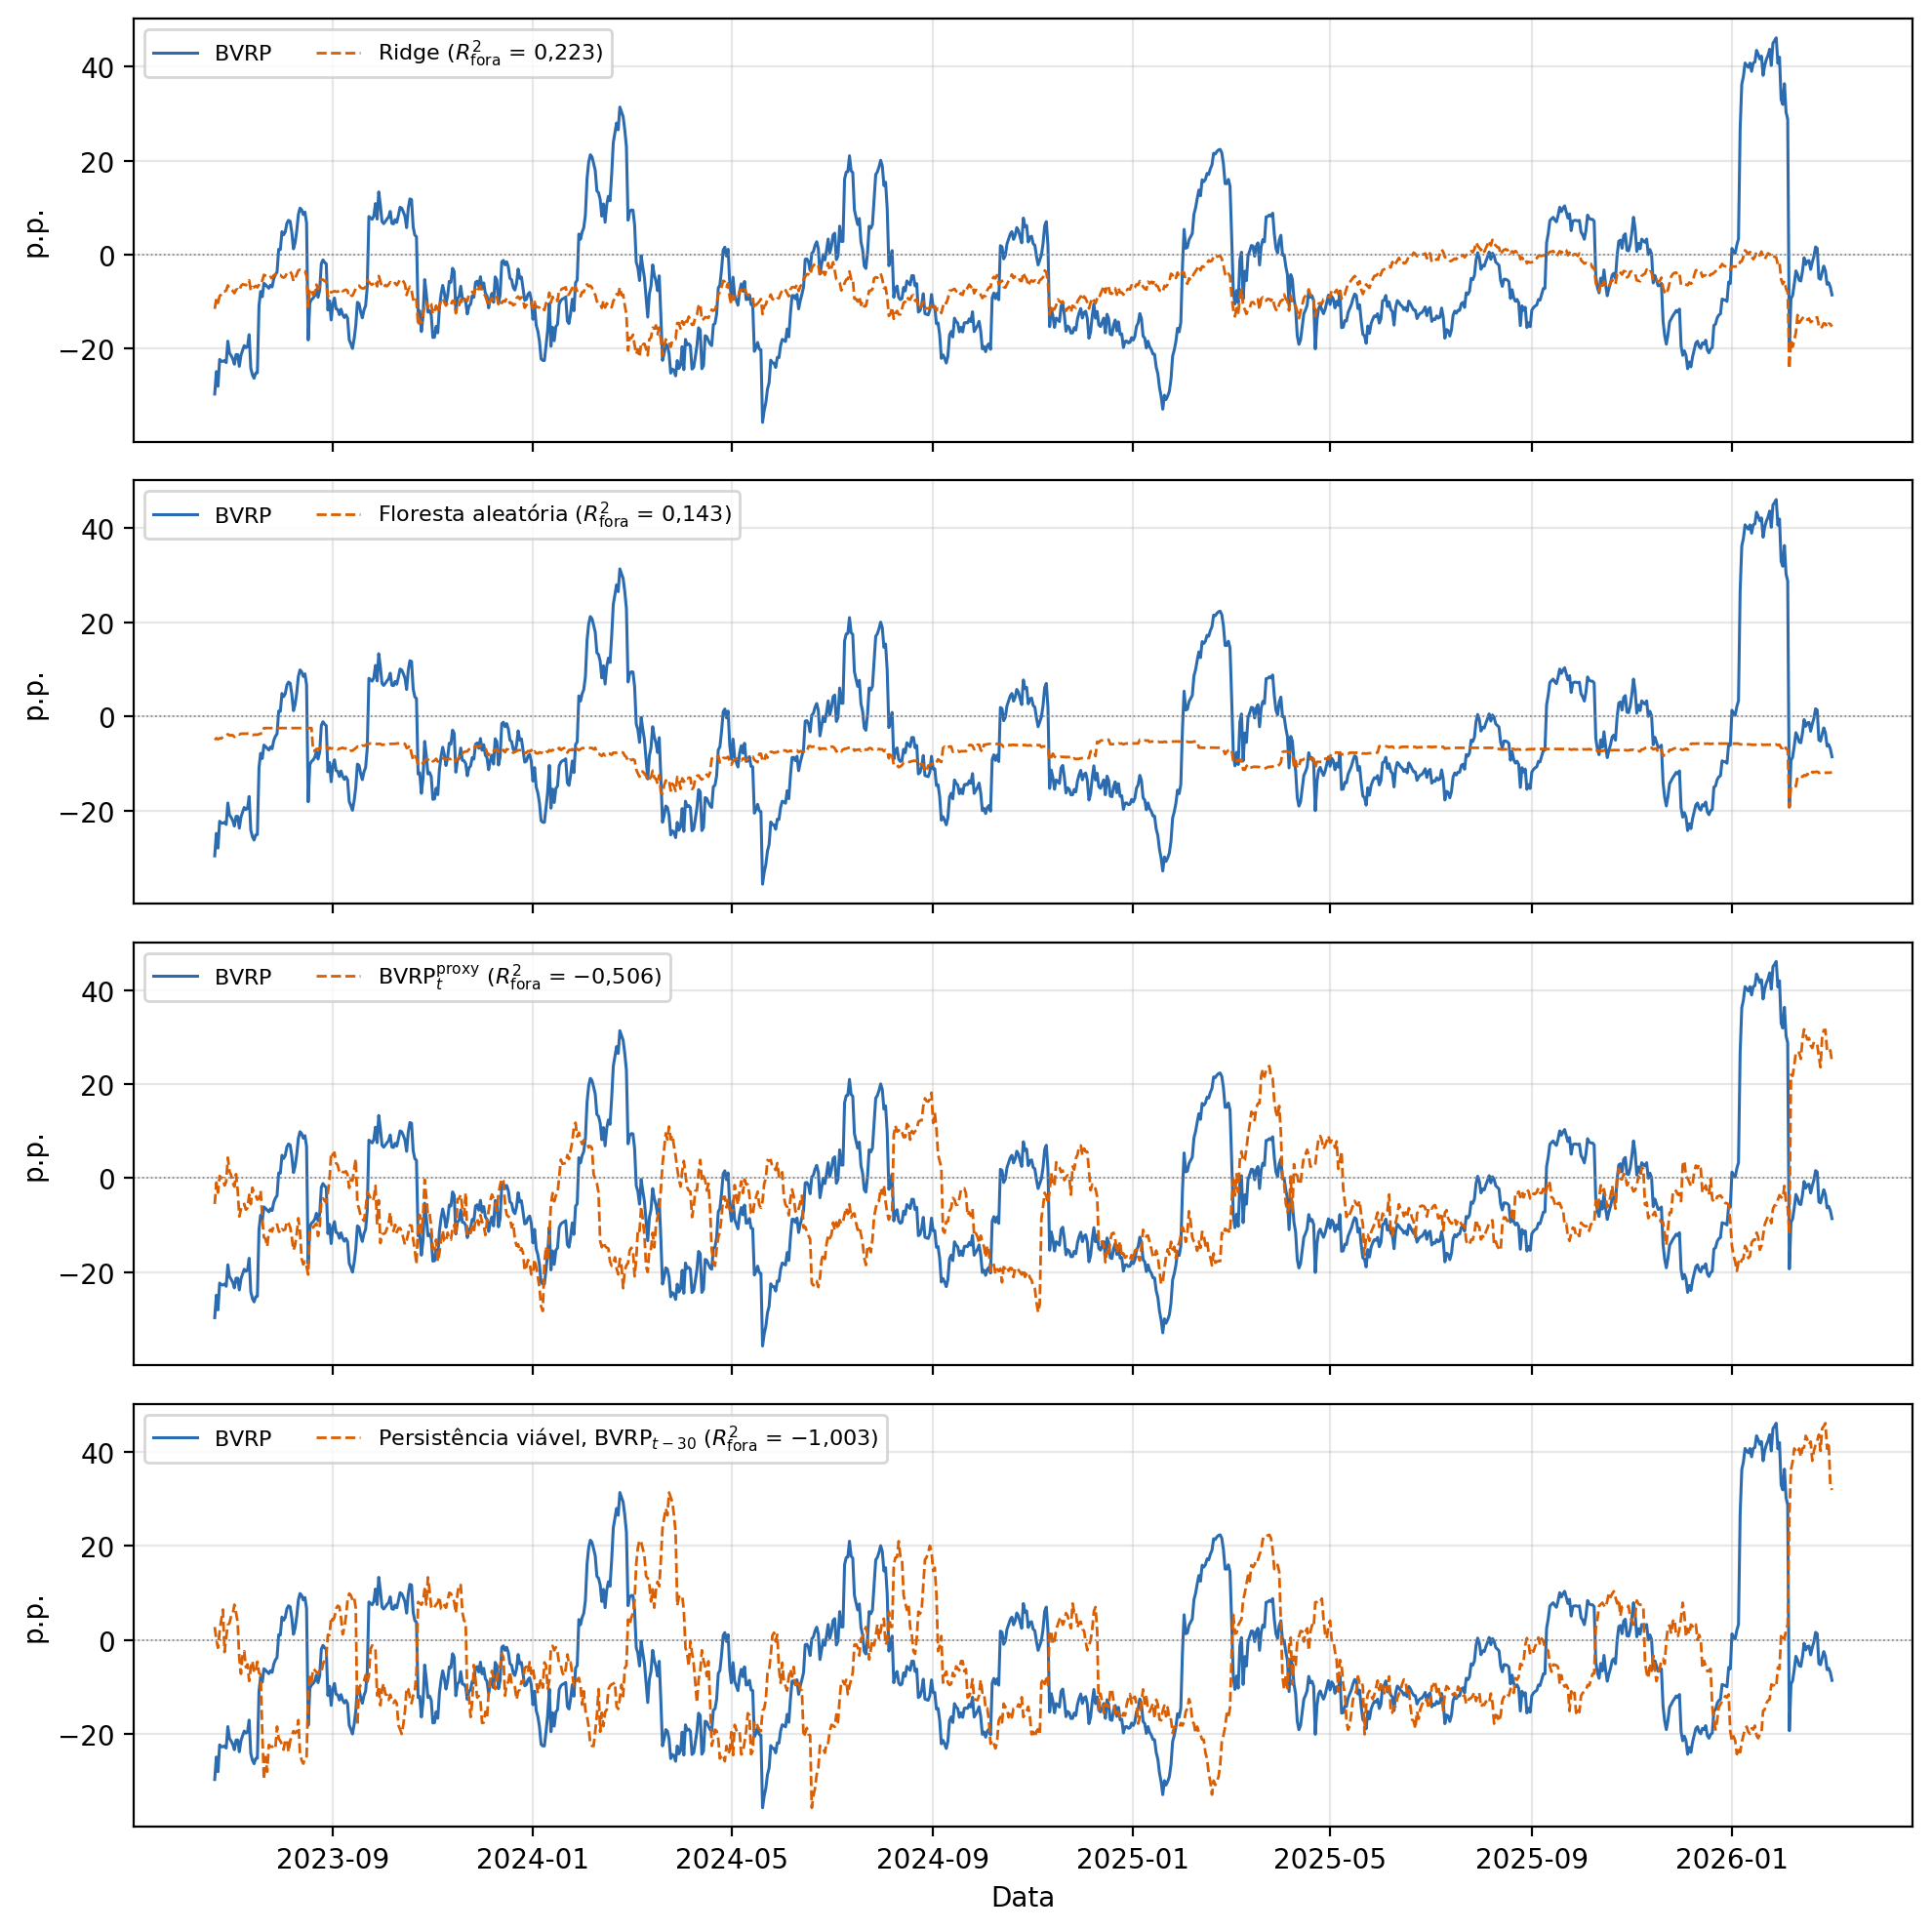
\includegraphics[width=0.95\linewidth]{figs/previsao_bvrp/fig_previsoes.png}
    \caption{BVRP e previsões fora da amostra (janela expansiva, 21/06/2023 a 03/03/2026): Ridge, floresta aleatória, $\text{BVRP}^{\text{proxy}}_t$ e prêmio realizado defasado, $\text{BVRP}_{t-30}$. Na legenda, o $R^2$ fora da amostra contra a média histórica.}
    \label{fig:prev-previsoes}
\end{figure}
}{}

Um teste placebo verifica a ausência de vazamento de informação futura: em
cada origem, o teste embaralha o alvo dentro do treino e reestima o modelo
(200 permutações nos lineares, 10 nas árvores). Se o procedimento não usa
informação do período de teste, o $R^2_{\text{fora}}$ com o alvo embaralhado
não deve ser positivo. As medianas ficam entre $-0{,}016$ e $0{,}000$ em todos
os modelos. O placebo não serve como teste de significância: as permutações
destroem a autocorrelação dos alvos sobrepostos, e a distribuição resultante
fica estreita demais; a significância vem dos testes acima.

% =========================================================
\section{Regularização em baixa dimensão}
\label{sec:prev-regularizacao}

Com 16 variáveis e de 760 a 1.720 observações de treino, o problema tem baixa
dimensão, e a motivação usual da regularização --- muitas variáveis em relação
ao número de observações --- não se aplica. Ainda assim, o Ridge supera o MQO
($R^2_{\text{fora}}$ de 0,223 contra 0,097; Diebold--Mariano entre os dois,
$p = 0{,}017$). A explicação está nas variáveis construídas. As volatilidades
históricas de janelas diferentes compartilham retornos; a proxy, sua variação e
o prêmio realizado defasado são combinações da volatilidade histórica e da IV.
Com regressores tão relacionados, os coeficientes do MQO têm variância alta: o
$R^2$ dentro da amostra do MQO (0,29) é três vezes o de fora (0,10). O Ridge
encolhe os coeficientes e, com eles, a previsão em direção à média histórica,
trocando viés por variância \citep{hastie2009elements}. Com sinal fraco, essa
troca compensa.

O LASSO vai além: zera todos os coeficientes em 12 das 33 origens e reproduz
a média histórica. Suas previsões diferem das do MQO em até 25,4 p.p., com
correlação de apenas 0,34. A regularização ajuda, portanto, não por selecionar
variáveis, mas por encolher a previsão para a média quando a informação das
variáveis é pouca.

% =========================================================
\section{Não linearidade e regimes de volatilidade}
\label{sec:prev-nao-linearidade}

A distribuição da volatilidade histórica de 30 dias é bimodal, e o corte de
$37{,}3\%$ a.a., estimado só na primeira janela, separa um regime de baixa e
um de alta volatilidade (Seção~\ref{sec:dados-regimes}). Se a relação entre as
variáveis e o prêmio muda entre os regimes, um modelo linear único é mal
especificado. Para testar essa hipótese, a dissertação estima o MQO com as 16
variáveis, a variável indicadora do regime de alta volatilidade, $D_t$, e as 16
interações $D_t X_t$, na amostra de modelagem inteira, com erro-padrão HAC de
31 defasagens. A Tabela~\ref{tab:prev-regime} reporta os resultados. As
interações são conjuntamente muito significantes: $\chi^2(16) = 94{,}9$, com
$p = 3 \times 10^{-13}$, e o mesmo vale com o corte reestimado em janela
expansiva ($\chi^2(16) = 85{,}6$). Dentro da amostra, há evidência de não
linearidade.

\begin{table}[H]
\centering
\small
\caption{Regime de volatilidade e previsão do BVRP.}
\label{tab:prev-regime}
\begin{tabular}{llrrr}
\toprule
Corte & $H_0$ & $\chi^2$ ($q$) & $p$ & $R^2$ dentro \\
\midrule
\multicolumn{5}{l}{\textit{Painel A: interações dentro da amostra (MQO, $N = 1.776$)}} \\
Corte fixo & 16 interações & 94{,}9 (16) & $3 \times 10^{-13}$ & 0{,}328 \\
Corte fixo & 16 interações e $D_t$ & 94{,}9 (17) & $8 \times 10^{-13}$ & 0{,}328 \\
Corte expansivo & 16 interações & 85{,}6 (16) & $2 \times 10^{-11}$ & 0{,}318 \\
Corte expansivo & 16 interações e $D_t$ & 86{,}9 (17) & $2 \times 10^{-11}$ & 0{,}318 \\
\addlinespace
\multicolumn{5}{l}{\textit{Painel B: previsão fora da amostra ($R^2_{\text{fora}}$, janela expansiva)}} \\
Modelo & Sem regime & Corte fixo & Corte expansivo & DM ($p$), fixo \\
\cmidrule(lr){1-5}
Ridge & 0{,}223 & 0{,}229 & 0{,}227 & 0{,}81 \\
MQO & 0{,}097 & $-$0{,}174 & $-$0{,}165 & 0{,}21 \\
\bottomrule
\end{tabular}
\par\smallskip
\parbox{0.95\linewidth}{\footnotesize\textit{Nota}: $D_t = 1$ se $\text{VH}_{t-29:t} > 37{,}3\%$ a.a. (corte fixo, estimado na primeira janela); no corte expansivo, reestimado em cada origem. Painel A: MQO com as 16 variáveis, $D_t$ e as 16 interações $D_t X_t$; estatística de Wald $\chi^2(q)$ com erro-padrão HAC de 31 defasagens. Painel B: modelos com as interações, mesmas origens do T5; DM: Diebold--Mariano bilateral contra o mesmo modelo sem regime.}
\end{table}


Essa evidência não se converte em previsão melhor. Com as interações, o
$R^2_{\text{fora}}$ do Ridge passa de 0,223 para 0,229, diferença que o
Diebold--Mariano não distingue de zero ($p = 0{,}81$); o do MQO, com 33
regressores, cai de 0,097 para $-0{,}174$. Os resultados são os mesmos com o
corte expansivo.

As árvores oferecem um teste mais flexível, porque não precisam de um corte
fixado de antemão: cada divisão escolhe a variável e o ponto de corte que mais
reduzem o erro, e as volatilidades entram em nível, de modo que uma árvore pode
encontrar sozinha o corte entre os regimes, ou outro qualquer. Mesmo assim, a
validação cruzada escolhe quase sempre árvores de um único corte
(Seção~\ref{sec:prev-modelos}), que não combinam variáveis, e as duas
famílias de árvores ficam abaixo do Ridge fora da amostra. A não linearidade
existe dentro da amostra, mas é fraca demais para melhorar a previsão do BVRP.
O Capítulo~\ref{chap:retornos_nao_linear} volta às árvores para a relação entre
o BVRP previsto e os retornos.

% =========================================================
\section{Síntese}
\label{sec:prev-sintese}

As variáveis disponíveis em $t$ contêm informação sobre o BVRP dos 30 dias
seguintes: os modelos superam a média histórica, e o Clark--West rejeita a
igualdade mesmo com a correção para múltiplas comparações. A previsibilidade é
modesta, e as previsões ficam próximas da média. O Ridge tem o melhor
desempenho, por encolher a previsão quando o sinal é fraco, e a não linearidade
encontrada dentro da amostra não melhora a previsão.

Os Capítulos~\ref{chap:retornos_linear} e~\ref{chap:retornos_nao_linear} usam
estas previsões, da janela expansiva, como regressor. A dissertação fixou a
escolha antes de ver os resultados dos retornos: o Ridge é a previsão principal do
Capítulo~\ref{chap:retornos_linear}, e a floresta aleatória, a do
Capítulo~\ref{chap:retornos_nao_linear}; em cada capítulo, o outro modelo serve
de teste de robustez. Como o BVRP previsto é um regressor gerado, a inferência
desses capítulos incorpora a incerteza da previsão
(Seção~\ref{sec:met-inferencia}).
